%%%%%%%%%%%%%%%%%%%%%%%%%%%%%%%%%%%%%%%%%%%%%%%%%%%%%%%%%%%%%%%%%%%%%%%%%%%
% Función: primeros pasos con la plantilla.
%
% Uso: modifica este fichero para adaptar el contenido a tu trabajo.
%%%%%%%%%%%%%%%%%%%%%%%%%%%%%%%%%%%%%%%%%%%%%%%%%%%%%%%%%%%%%%%%%%%%%%%%%%%

\chapter{Primeros pasos}
\label{cha:primeros-pasos}

En este capítulo te acompaño desde la descarga de la plantilla hasta la generación del primer PDF. Primero encontrarás los archivos publicados y los ejemplos, después prepararás tu entorno y compilarás la plantilla sin modificarla para comprobar que funciona. A continuación podrás introducir tus datos, conocer el anteproyecto y preparar una estructura mínima para escribir tu trabajo. Al final te explico cómo registrar sus fuentes en Git. Puedes trabajar desde tu editor habitual de \LaTeX{} o con Overleaf, sin utilizar una terminal ni conocer el \texttt{Makefile}.

\section{Descarga y documentos de ejemplo}
\label{sec:descarga-ejemplos}

La \href{https://www.dropbox.com/sh/mm6fwh3ruuuyjz2/AABDUmo7Xj1S968FeJgbmFPva?dl=0}{carpeta de descargas de la plantilla} contiene los archivos ZIP y TGZ de la versión publicada y una selección reducida de documentos completos. Te recomendamos comenzar por \texttt{TFG-GIEC-spanish.pdf}, que utiliza la estructura y el estilo predeterminados. El fichero \texttt{01-DOWNLOAD-GUIDE.pdf}, situado al principio de la carpeta, enumera todos los ejemplos disponibles y explica qué idioma, estructura, estilo tipográfico y cubierta muestra cada uno.

Los PDF precompilados son ejemplos representativos y no una copia para cada titulación admitida. Si no encuentras un documento dedicado a tu grado o máster, no significa que no esté soportado: consulta los identificadores disponibles en \texttt{Config/myconfig.tex} y la lista descrita en el capítulo~\ref{cha:configuracion}. El fichero \texttt{RELEASE.txt} de la carpeta te permite comprobar a qué versión corresponden los archivos publicados.

Para empezar a escribir, descarga la distribución ZIP o TGZ y descomprímela en una carpeta en la que tengas permisos de escritura. Conserva juntos sus directorios: \texttt{Book/} necesita los archivos compartidos de \texttt{Config/}. El repositorio completo incluye además herramientas de mantenimiento y material histórico que no necesitas para utilizar la plantilla.

\section{Prerrequisitos}
\label{sec:prerrequisitos}

Para empezar te recomiendo trabajar en tu equipo con una distribución de \LaTeX{} completa y actualizada y el editor \href{https://www.texstudio.org/}{\texttt{TeXstudio}}. Si ya utilizas otro editor, puedes seguir haciéndolo. También puedes trabajar desde el navegador con \texttt{Overleaf}, sin instalar una distribución ni un editor en tu equipo\footnote{Antes de subir tu proyecto a un servicio en línea, revisa sus condiciones de privacidad y, si utilizas funciones de IA, los controles de uso de datos. Si contiene información confidencial, datos personales o material sujeto a acuerdos con terceros, consulta primero con tu tutor o institución. Una instalación local permite trabajar sin subir el proyecto a estos servicios.}. La sección~\ref{sec:entorno-navegador} describe sus requisitos y limitaciones, y la sección~\ref{sec:compilacion-navegador} explica cómo generar tu primer PDF con esta opción.

La plantilla utiliza \texttt{biber} para preparar la bibliografía. Las distribuciones indicadas a continuación proporcionan esa herramienta, y solo tendrás que seleccionarla en el editor como se explica en la sección~\ref{sec:configurar-texstudio}. No necesitas aprender a ejecutarla por separado para seguir este recorrido.

\subsection{Windows}

En Windows puedes utilizar \texttt{MiKTeX} o \texttt{TeX Live}. Si empiezas desde cero, este es el procedimiento que te recomiendo:

\begin{itemize}
  \item Instala la versión actual de \href{https://miktex.org/download}{\texttt{MiKTeX}} y permite que instale los paquetes que falten, automáticamente o tras preguntarte.
  \item Abre \texttt{MiKTeX Console}, ejecuta \texttt{Check for updates} e instala las actualizaciones disponibles.
  \item Instala \href{https://www.texstudio.org/}{\texttt{TeXstudio}} y sigue la configuración común de la sección~\ref{sec:configurar-texstudio}.
\end{itemize}

La generación automática de acrónimos y símbolos se ha comprobado con \texttt{MiKTeX} y \texttt{TeXstudio} en Windows 11, sin instalar \texttt{perl} por separado. La sección~\ref{sec:compilacion} explica cómo comprobar el resultado. Si más adelante quieres utilizar el \texttt{Makefile}, necesitarás un entorno compatible con sus herramientas, como WSL, pero no hace falta para seguir las instrucciones del editor.

Parte de estas instrucciones se basa en la información que nos proporcionó Cristina Losada sobre la configuración de TeXmaker en Windows. Muchas gracias por su ayuda.

\subsection{GNU/Linux}

En Ubuntu o Debian, busca estos nombres exactos en el gestor de paquetes de tu sistema:

\begin{itemize}
  \item \texttt{texlive-full}: instala la distribución completa de \LaTeX{}, con sus paquetes, fuentes e idiomas. Ocupa varios gigabytes y puede tardar en instalarse, pero evita que tengas que averiguar qué paquetes individuales necesita la plantilla.
  \item \texttt{texstudio}: instala el editor en el que escribirás tu trabajo.
  \item \texttt{biber}: instala la herramienta que prepara la bibliografía. Con \texttt{texlive-full} normalmente ya quedará instalada como dependencia, pero puedes comprobarlo en el gestor.
\end{itemize}

Si tienes el gestor de paquetes \texttt{Synaptic}, ábrelo, busca cada nombre, selecciona \texttt{Marcar para instalar} y pulsa \texttt{Aplicar}. Acepta también las dependencias que proponga. \texttt{Synaptic} no viene instalado en todas las versiones de Ubuntu. La \href{https://help.ubuntu.com/stable/ubuntu-help/addremove-install-synaptic.html.en}{ayuda de Ubuntu sobre \texttt{Synaptic}} explica cómo obtenerlo y utilizarlo.

En otras distribuciones GNU/Linux, instala \texttt{TeX Live}, \texttt{TeXstudio} y \texttt{biber} mediante su gestor de paquetes. Los nombres de las colecciones pueden ser distintos. Después sigue la configuración de la sección~\ref{sec:configurar-texstudio}. Si prefieres instalar desde la terminal, encontrarás los comandos y una alternativa de instalación más reducida en la sección~\ref{sec:instalacion-gnu-linux}.

\subsection{macOS}

En macOS puedes utilizar \texttt{MacTeX} junto con \texttt{TeXstudio}, \texttt{TeXShop} u otro editor compatible. Para seguir el recorrido recomendado, prepara estas dos aplicaciones:

\begin{itemize}
  \item Instala \href{https://www.tug.org/mactex/}{\texttt{MacTeX}}. La instalación completa ya proporciona \texttt{biber}.
  \item Instala \href{https://www.texstudio.org/}{\texttt{TeXstudio}} y sigue la configuración de la sección~\ref{sec:configurar-texstudio}.
\end{itemize}

Las primeras comprobaciones de la generación de glosarios en macOS fueron realizadas y compartidas con nosotros por Carlos Cruz. Muchas gracias por su ayuda.

\subsection{Configuración de \texttt{TeXstudio}}
\label{sec:configurar-texstudio}

Solo tienes que seleccionar \texttt{biber} como herramienta bibliográfica. La configuración es la misma para Windows, GNU/Linux y macOS:

\begin{itemize}
  \item Abre \texttt{Opciones} > \texttt{Configurar TeXstudio}. En macOS, abre \texttt{TeXstudio} > \texttt{Preferencias}.
  \item Entra en \texttt{Compilar} y selecciona \texttt{Biber} en \texttt{Herramienta bibliográfica por defecto}, como muestra la figura~\ref{fig:texstudio-biber-config}.
  \item Confirma los cambios con \texttt{Aceptar}.
\end{itemize}

Si los menús están en inglés, busca \texttt{Options} > \texttt{Configure TeXstudio} (o \texttt{TeXstudio} > \texttt{Preferences} en macOS) y después \texttt{Build} > \texttt{Default Bibliography Tool} > \texttt{Biber}.

\begin{figure}[htbp]
  \centering
  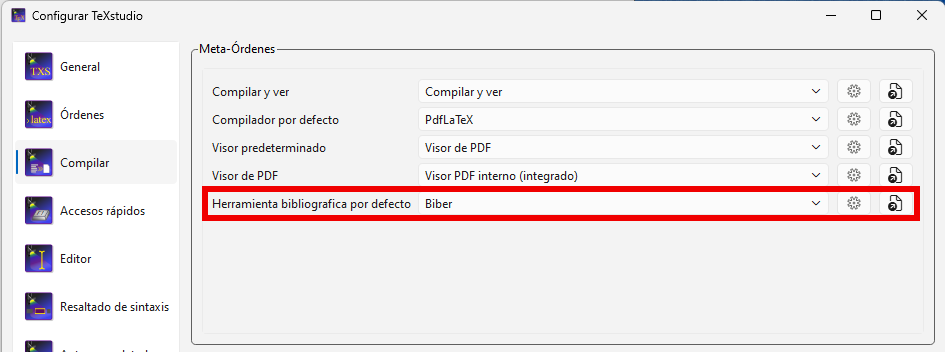
\includegraphics[width=\linewidth]{manual/texstudio-biber-config.png}
  \caption{Selección de \texttt{Biber} como herramienta bibliográfica por defecto en \texttt{TeXstudio}.}
  \label{fig:texstudio-biber-config}
\end{figure}

\texttt{TeXstudio} utiliza \texttt{pdflatex} de forma predeterminada. Si no has cambiado el compilador, puedes dejarlo como está. Si utilizas otro editor, selecciona \texttt{biber} como procesador bibliográfico y comprueba que su compilador sea \texttt{pdflatex}.

\subsection{Si prefieres trabajar desde el navegador}
\label{sec:entorno-navegador}
\label{sec:entorno-overleaf}

Esta alternativa te permite trabajar sin instalar \LaTeX{} en tu equipo. Revisa los requisitos y limitaciones del servicio antes de subir tu proyecto, y ten en cuenta la nota sobre privacidad de la sección~\ref{sec:prerrequisitos}.

Con \href{https://www.overleaf.com/}{\texttt{Overleaf}} puedes trabajar desde el navegador. Sólo necesitas una cuenta y conexión a Internet. Su guía de primeros pasos puede servirte de apoyo~\cite{overleaf-first-project}.

Ojo: con el plan gratuito es casi seguro que no podrás compilar el manual completo porque el tiempo disponible es muy limitado. Si se agota, no significa que hayas hecho algo mal. Puedes utilizar una instalación local o, después de revisar el manual precompilado, probar con la estructura mínima de la sección~\ref{sec:estructura-minima} y prescindir del material de ejemplo que no necesites. Un documento más pequeño puede caber en el límite de tiempo, pero no puedo garantizártelo.

La sección~\ref{sec:compilacion-overleaf} explica cómo importar la distribución y compilarla.

\subsection{Si te manejas con la terminal: herramientas opcionales para \texttt{make}}

\texttt{make} permite automatizar tareas, pero tu editor es una alternativa igualmente válida. Para utilizar el \texttt{Makefile} suministrado necesitas, además de la distribución de \LaTeX{} y \texttt{biber}, las herramientas \texttt{make}, \texttt{bash}, \texttt{latexmk}, \texttt{perl} y \texttt{makeglossaries}. El objetivo predeterminado utiliza también \texttt{Ghostscript} para generar una copia comprimida. Encontrarás el procedimiento y las herramientas adicionales para convertir figuras y diagramas en la sección~\ref{sec:compilacion-makefile}.

Puedes ampliar estas indicaciones con la documentación del proyecto \LaTeX{}~\cite{latex-project-docs} y el manual de \texttt{biber}~\cite{biber-manual}, pero no necesitas ni mucho menos leerlos completos para empezar.

\section{Compilación del documento principal}
\label{sec:compilacion}

Haz la primera compilación antes de modificar ningún archivo. Así podrás comprobar que tu entorno funciona y consultar el manual completo y sus ejemplos. Después introducirás tus datos en \texttt{Config/myconfig.tex} y volverás a compilar para revisar la personalización, como se explica en la sección~\ref{sec:primera-personalizacion}.

\subsection{Desde tu editor}
\label{sec:compilacion-editor}

Abre \texttt{Book/book.tex} en \texttt{TeXstudio} y selecciona \texttt{Herramientas} > \texttt{Compilar y ver} (\texttt{F5}), o pulsa el icono de la doble flecha verde \raisebox{-0.15em}{
\includegraphics[height=1em]{manual/texstudio-build-and-view-16.png}} de la barra de herramientas. Si utilizas otro editor, abre ese mismo archivo y utiliza su función habitual de construcción. Cuando escribas en un capítulo, sigue compilando \texttt{Book/book.tex}, no el archivo del capítulo por separado.

La plantilla utiliza la opción \texttt{automake} del paquete \texttt{glossaries} para ejecutar \texttt{makeindex} automáticamente y preparar las listas de acrónimos y símbolos. Si tu distribución permite esa ejecución, no necesitas instalar \texttt{perl} ni ejecutar el script \texttt{makeglossaries} para compilar desde el editor. Si las listas no aparecen después de la primera compilación, vuelve a compilar. Si siguen sin actualizarse, comprueba los mensajes de \texttt{makeindex} en el registro antes de instalar herramientas adicionales. La vía opcional mediante el \texttt{Makefile} utiliza \texttt{makeglossaries}, como se explica en la sección~\ref{sec:compilacion-makefile}.

Si recibes un aviso de que falta un fichero \texttt{.sty}, instala el paquete correspondiente desde tu distribución de \LaTeX{}. En \texttt{MiKTeX} puedes permitir la instalación automática de paquetes. Para otras incidencias, consulta la sección~\ref{sec:problemas-conocidos} antes de cambiar otros archivos.

El PDF resultante es este manual y una colección de ejemplos. Revísalo para orientarte, sin necesidad de leerlo entero. Cuando todo funcione, continúa con la sección~\ref{sec:primera-personalizacion}.

\subsection{Si trabajas desde el navegador}
\label{sec:compilacion-navegador}
\label{sec:compilacion-overleaf}

Después de descargar la distribución, utiliza el ZIP sin descomprimir para importar el proyecto en \texttt{Overleaf}. Antes de empezar, revisa sus requisitos y limitaciones en la sección~\ref{sec:entorno-overleaf}.

Para importar y compilar la plantilla sigue estos pasos:

\begin{itemize}
  \item Inicia sesión y selecciona \texttt{New Project} > \texttt{Upload Project}.
  \item Sube sin descomprimir el ZIP de la distribución, disponible en la \href{https://www.dropbox.com/sh/mm6fwh3ruuuyjz2/AABDUmo7Xj1S968FeJgbmFPva?dl=0}{carpeta de descargas de la plantilla}.
  \item Abre \texttt{Settings} > \texttt{Compiler} > \texttt{Main document} y selecciona \texttt{Book/book.tex}.
  \item Comprueba que el compilador sea \texttt{pdfLaTeX} y pulsa \texttt{Recompile}.
\end{itemize}

\texttt{Overleaf} gestiona la cadena de construcción, incluida la bibliografía, sin que tengas que configurar \texttt{biber} por separado ni ejecutar el \texttt{Makefile}. Comprueba que aparezcan las referencias y los listados de acrónimos y símbolos. Si alguno no se actualiza, revisa el documento principal seleccionado y prueba a recompilar el proyecto desde cero.

Si se agota el tiempo de compilación, revisa el aviso de la sección~\ref{sec:entorno-overleaf}.

Para compilar otro documento independiente, como \texttt{Anteproyecto/anteproyecto.tex} o un formulario administrativo, selecciónalo en el mismo campo \texttt{Main document}. Para trabajar en los capítulos del libro, mantén seleccionado \texttt{Book/book.tex}.

Después continúa con la primera personalización de la sección~\ref{sec:primera-personalizacion}.

\section{Los archivos que realmente necesitas conocer}
\label{sec:archivos-esenciales}

La separación en carpetas no busca complicarte el trabajo, sino mantener cada elemento en su sitio para que puedas encontrarlo con facilidad. La mayoría de los archivos cumplen una función concreta y no tendrás que ocuparte de todos a la vez.

Al principio basta con localizar estos archivos:

\begin{itemize}
  \item \texttt{Config/myconfig.tex}: donde encontrarás los datos y las opciones generales del documento.
  \item \texttt{Book/book.tex}: donde encontrarás el documento principal que debes compilar, aunque normalmente no tendrás que editarlo.
  \item \texttt{Book/content-standard.tex}: donde encontrarás la organización de los capítulos, la bibliografía y los apéndices.
  \item \texttt{Book/biblio/biblio.bib}: donde encontrarás las referencias bibliográficas.
\end{itemize}

Y estas carpetas, donde irás guardando el contenido de tu trabajo:

\begin{itemize}
  \item \texttt{Book/chapters/}: donde encontrarás los capítulos del trabajo.
  \item \texttt{Book/abstract/}: donde encontrarás el resumen y el abstract.
  \item \texttt{Book/appendix/}: donde encontrarás los apéndices.
  \item \texttt{Book/figures/}: donde encontrarás las figuras e imágenes.
  \item \texttt{Book/diagrams/}: donde encontrarás los diagramas editables o generados.
\end{itemize}

Por ahora, céntrate en estos archivos y carpetas. Los demás pueden esperar. El capítulo~\ref{cha:estructura-documento} describe la estructura completa para cuando necesites consultarla. Encontrarás los archivos que debes compilar para el anteproyecto y los formularios en el capítulo~\ref{cha:documentos-complementarios}. Solo si preparas una tesis doctoral por compendio utilizarás \texttt{Book/content-compendium.tex} para organizar su contenido, como se explica en la sección~\ref{sec:tesis-compendio}.

\section{Primera personalización}
\label{sec:primera-personalizacion}

Una vez que hayas compilado la plantilla sin modificarla, abre \texttt{Config/myconfig.tex} y utiliza la búsqueda de tu editor para localizar las definiciones siguientes. No necesitas conocer sus números de línea, que pueden cambiar entre versiones. En una definición como la del ejemplo, cambia solo el contenido del último par de llaves:

\begin{verbatim}
\newcommand{\myDegree}{GIEC}
\end{verbatim}

Para esta primera prueba basta con revisar estos datos:

\begin{itemize}
  \item Titulación: busca \texttt{\textbackslash{}myDegree} y sustituye \texttt{GIEC} por el identificador de tu titulación. Encontrarás las opciones disponibles en los comentarios inmediatamente anteriores a su definición.
  \item Idioma: busca \texttt{\textbackslash{}myLanguage} y elige \texttt{spanish} o \texttt{english}.
  \item Título: busca \texttt{\textbackslash{}myBookTitleSpanish} y \texttt{\textbackslash{}myBookTitleEnglish} y sustituye los títulos de ejemplo por los de tu trabajo. La plantilla selecciona el que corresponde al idioma, aunque algunas páginas institucionales utilizan ambos.
  \item Autoría: completa \texttt{\textbackslash{}myAuthorName} y \texttt{\textbackslash{}myAuthorSurname}. En \texttt{\textbackslash{}myAuthorGender}, indica \texttt{male} o \texttt{female} para adaptar el género gramatical.
  \item Tutoría: completa \texttt{\textbackslash{}myAcademicTutorFullName} y \texttt{\textbackslash{}myAcademicTutorGender}. Si tienes cotutor, completa también \texttt{\textbackslash{}myCoTutorFullName} y \texttt{\textbackslash{}myCoTutorGender}. Si no, deja vacío el último par de llaves de la definición de su nombre: \texttt{\{\}}.
\end{itemize}

No elimines ni comentes las definiciones de variables. Cuando un dato opcional no corresponda a tu caso, conserva la variable y deja su valor vacío. Puedes completar las fechas cuando las conozcas, sin tener que inventar ahora una fecha de defensa. El capítulo~\ref{cha:configuracion} contiene la referencia completa para cuando necesites otros campos y opciones.

Vuelve a compilar \texttt{Book/book.tex} y comprueba que aparecen tu nombre, el título y la titulación correctos. Revisa también los nombres de los tutores y las fechas que hayas introducido si el modelo de tu titulación muestra esos datos, como ocurre en los modelos de la UAH. No dejes los datos de ejemplo en la versión que entregues. Cuando hayas verificado el resultado y revisado el manual, podrás preparar la estructura mínima de la sección~\ref{sec:estructura-minima} para comenzar a escribir. Si antes necesitas un anteproyecto, encontrarás su punto de entrada a continuación.

\section{Trabajo con el anteproyecto}
\label{sec:primeros-pasos-anteproyecto}

Si antes de comenzar la memoria necesitas preparar un anteproyecto, utiliza \texttt{Anteproyecto/anteproyecto.tex} como documento principal. Esta plantilla reutiliza los datos definidos en \texttt{Config/myconfig.tex} y puedes compilarla con tu editor habitual o mediante su \texttt{Makefile} opcional. Si trabajas en línea, selecciona ese fichero como se explica para \texttt{Overleaf} en la sección~\ref{sec:compilacion-overleaf}. Encontrarás una descripción más completa de su contenido y compilación en la sección~\ref{sec:plantilla-de-anteproyecto}.

\section{Preparación de una estructura mínima}
\label{sec:estructura-minima}

Ya puedes escribir en la plantilla tal como está, pero sus capítulos contienen este manual y los ejemplos. Para empezar tu trabajo sin tener que retirarlos uno a uno, puedes sustituirlos por una estructura mínima con capítulos casi vacíos. Esta preparación es opcional: conserva la organización actual si prefieres adaptarla por tu cuenta.

Después de completar la primera compilación y la personalización de la sección~\ref{sec:compilacion}, guarda una copia de seguridad de la carpeta completa, incluyendo cualquier contenido que hayas escrito, por si algo sale mal. Hazlo antes de sustituir o eliminar archivos, tanto si utilizas el método manual como si recurres a \texttt{make}.

Cuando hayas preparado la estructura mínima con cualquiera de los dos métodos siguientes, organiza tu trabajo añadiendo, eliminando o reordenando las instrucciones \texttt{\textbackslash{}input\{...\}} de \texttt{Book/content-standard.tex}. Escribe en los archivos de contenido, sigue compilando \texttt{Book/book.tex} y revisa el PDF y los avisos. Hacer cambios pequeños y compilar con frecuencia facilita encontrar los errores.

\subsection{Método manual}
\label{sec:estructura-minima-manual}

Para preparar una memoria convencional, utiliza los capítulos y apéndices casi vacíos de \texttt{Book/chapters/bare/} y \texttt{Book/appendix/bare/}. Sigue estos pasos desde la carpeta raíz de la plantilla:

\begin{itemize}
  \item Comprueba que has guardado la copia de seguridad.
  \item Elimina solo los ficheros \texttt{.tex} situados directamente en \texttt{Book/chapters/} y \texttt{Book/appendix/}. No elimines las carpetas ni sus subcarpetas, como \texttt{bare/}, \texttt{orig/} o \texttt{compendium/}, ni los archivos de otros tipos. Esta limpieza no es necesaria para compilar, pero evita que confundas los ejemplos con el contenido que vas a utilizar.
  \item Copia a \texttt{Book/chapters/} los ficheros de capítulo de \texttt{Book/chapters/bare/}, excepto el archivo de organización \texttt{content-standard.tex}.
  \item Copia a \texttt{Book/appendix/} los ficheros de \texttt{Book/appendix/bare/}.
  \item Copia el archivo de organización \texttt{content-standard.tex} de \texttt{Book/chapters/bare/} a \texttt{Book/}, sustituyendo el existente. Este fichero ya incluye los capítulos y apéndices mínimos que acabas de copiar.
  \item Revisa en \texttt{Config/myconfig.tex} qué elementos opcionales quieres incluir y deja en \texttt{false} los que todavía no necesites. Por ejemplo, los índices de vídeos y símbolos suelen ser prescindibles al empezar. Encontrarás la referencia de estas opciones en la sección~\ref{sec:elementos-opcionales-configuracion}.
  \item Compila de nuevo \texttt{Book/book.tex}.
\end{itemize}

\subsection{Si te sientes cómodo con la terminal}
\label{sec:estructura-minima-make}

Si utilizas \texttt{make}, ejecuta \texttt{make bare} desde \texttt{Book/}. Con la estructura convencional predeterminada, este objetivo crea una copia de seguridad, instala los capítulos, apéndices y el fichero \texttt{content-standard.tex} mínimos, y desactiva parte del material opcional de ejemplo. También ofrece eliminar figuras y diagramas de ejemplo, solo si lo confirmas. Antes de ejecutarlo, comprueba igualmente que has guardado tu propia copia de seguridad. La sección~\ref{sec:compilacion-makefile} describe los requisitos y los objetivos disponibles, incluido \texttt{make bare-standard}.

\subsection{Caso particular: tesis por compendio de publicaciones}

Solo si vas a preparar una tesis doctoral por compendio debes seleccionar \texttt{compendium}. En ese caso elimina los ficheros \texttt{.tex} situados directamente en \texttt{Book/chapters/compendium/}, copia allí los seis capítulos de \texttt{Book/chapters/compendium/bare/}, sin copiar el fichero \texttt{content-compendium.tex}, y utiliza este último para sustituir \texttt{Book/content-compendium.tex}. El objetivo \texttt{make bare} realiza esas operaciones automáticamente cuando detecta esa estructura. La versión completa distribuida se conserva en \texttt{Book/chapters/compendium/orig/} y puedes restaurarla mediante \texttt{make orig-compendium}. Consulta la sección~\ref{sec:tesis-compendio} para conocer la organización de las dos partes y la forma de incorporar las publicaciones.

\section{Preparación del repositorio Git}
\label{sec:preparacion-repositorio-git}

\texttt{git} guarda el historial de tu proyecto en un repositorio y te permite recuperar versiones anteriores. Cada \emph{commit} registra un conjunto de cambios con un mensaje que los describe. No lo necesitas para compilar, pero te lo recomiendo para no depender de copias llamadas ``final'', ``final-bueno'' y ``ahora-sí-final''.

El historial se conserva en tu equipo. Puedes compartir una copia remota mediante \texttt{GitHub}, \texttt{GitLab} u otro servicio, pero recuerda sincronizar tus cambios para mantenerla al día. Puedes consultar la documentación de \texttt{git}~\cite{git-manual} cuando quieras profundizar, aunque utilices una aplicación gráfica.

Después de comprobar la compilación y preparar el contenido con el que vas a trabajar, puedes crear el repositorio y hacer el primer \emph{commit}. No es obligatorio utilizar la estructura mínima para hacerlo. La vía gráfica de la sección~\ref{sec:primer-commit-grafico} es suficiente para empezar. Más adelante encontrarás la lista detallada de ficheros y la alternativa de sincronización mediante \texttt{make}.

Si has descargado la distribución ZIP o TGZ, encontrarás en su raíz un \texttt{README.md} preparado para describir tu trabajo. Antes del primer commit, sustituye sus textos entre corchetes por el título, la autoría, la titulación, el centro, los tutores, el curso y una breve descripción, y elimina las líneas opcionales que no necesites. Este fichero presenta tu proyecto en el repositorio, pero no configura la compilación: los datos del documento siguen definiéndose en \texttt{Config/myconfig.tex}.

\subsection{Primer commit mediante una aplicación gráfica}
\label{sec:primer-commit-grafico}

La forma más sencilla de preparar el primer commit sin utilizar la línea de comandos consiste en partir de la distribución oficial y conservar el fichero \texttt{.gitignore} incluido en su directorio raíz. Este fichero indica a Git qué auxiliares, resultados de compilación y ficheros temporales debe ignorar, y las aplicaciones gráficas habituales respetan esas reglas.

Puedes utilizar \texttt{GitHub Desktop}, el panel de control de versiones de \texttt{Visual Studio Code}, \texttt{GitKraken}, \texttt{Sourcetree} u otro cliente gráfico. Aunque cambien los nombres y la presentación, puedes preparar el primer \emph{commit} sin elegir los cientos de ficheros uno a uno. Sigue este procedimiento:

\begin{itemize}
  \item Abre como repositorio la carpeta raíz de la plantilla, en la que se encuentran \texttt{README.md}, \texttt{Config/} y \texttt{Book/}. Si todavía no es un repositorio, utiliza la opción de la aplicación para crear o inicializar uno en esa carpeta.
  \item Conserva el fichero \texttt{.gitignore} incluido en la plantilla. Se encarga de excluir los auxiliares de compilación, los PDF generados y los temporales habituales.
  \item Selecciona todos los archivos que te proponga la aplicación. La opción puede llamarse \texttt{Stage all}, \texttt{Stage all changes}, \texttt{Select all} o aparecer como una casilla para marcarlos todos. Aunque haya muchos, no tienes que elegirlos uno a uno. Si aparecen archivos personales que hayas copiado a esa carpeta y no quieras compartir, desmárcalos.
  \item Escribe un mensaje que describa el inicio de tu trabajo y crea el \emph{commit}. Publicarlo o sincronizarlo posteriormente con \texttt{GitHub}, \texttt{GitLab} u otro servidor es una operación separada y opcional.
\end{itemize}

Este procedimiento resulta especialmente apropiado para un repositorio nuevo creado desde la distribución oficial. Si un fichero ya estaba versionado, \texttt{.gitignore} no deja de versionarlo por sí solo. En los siguientes \emph{commits}, revisa los cambios que quieras registrar. No fuerces la inclusión de un fichero ignorado sin comprobar primero por qué coincide con una regla de \texttt{.gitignore}.

\subsection{Ficheros que debes versionar}
\label{sec:ficheros-versionar}

En el primer commit debes incluir los siguientes tipos de ficheros:

\begin{itemize}
  \item Los ficheros de configuración compartida de \texttt{Config/}, en particular \texttt{myconfig.tex}, y los ficheros estructurales que cargan tus documentos.
  \item \texttt{Book/book.tex}, \texttt{Book/content-standard.tex} o, en el caso especializado, \texttt{Book/content-compendium.tex}, además de los capítulos, apéndices, resúmenes, bibliografía y demás fuentes \texttt{.tex} o \texttt{.bib} que utilice realmente el libro.
  \item \texttt{Anteproyecto/anteproyecto.tex} y los formularios de \texttt{PapeleoTFG/}, \texttt{PapeleoTFM/} o \texttt{PapeleoPHD/} que quieras poder generar.
  \item Las figuras, diagramas, logotipos, cartas y otros recursos que los documentos lean durante la compilación. Esto incluye los PDF que sean recursos de entrada, por ejemplo una carta incorporada mediante \texttt{\textbackslash{}includepdf}.
  \item Los \texttt{Makefile}, los ficheros \texttt{.gitignore}, el fichero \texttt{README.md}, la licencia y cualquier script propio que necesites para reconstruir los documentos.
\end{itemize}

A medida que avances, añade los nuevos capítulos, referencias bibliográficas, figuras, datos o scripts que incorpores al trabajo y registra también la eliminación de los que dejes de utilizar. Antes de cada commit, revisa la lista de cambios que muestra tu cliente de Git y selecciona los ficheros que correspondan. Si trabajas desde la línea de comandos, puedes consultar \texttt{git status}, añadir rutas concretas mediante \texttt{git add} y retirar únicamente del índice un fichero que quieras conservar en tu equipo mediante \texttt{git rm --cached}.

No debes subir nunca los auxiliares creados durante la compilación, como los ficheros \texttt{.aux}, \texttt{.log}, \texttt{.fls}, \texttt{.fdb\_latexmk}, \texttt{.synctex.gz}, \texttt{.bcf}, \texttt{.blg}, \texttt{.bbl}, \texttt{.run.xml}, \texttt{.toc}, \texttt{.lof} o \texttt{.lot}; ni tampoco los archivos temporales del editor, los paquetes de distribución ni los PDF generados del libro, el anteproyecto o el papeleo. Como excepción, puedes conservar la versión final definitiva del documento si existe una razón clara para versionarla, pero no acumules en Git los PDF de cada compilación.

\subsection{Sincronización mediante el \texttt{Makefile}}

Antes de utilizar este objetivo debes trabajar dentro de un repositorio Git, bien porque hayas clonado la plantilla desde GitHub u otro servidor, bien porque hayas creado un repositorio local en la carpeta raíz mediante \texttt{git init .}. Después de preparar y confirmar el primer commit podrás configurar un repositorio remoto y publicarlo mediante \texttt{git push}.

Si dispones de \texttt{make} y Bash, ejecuta desde el directorio raíz del proyecto:

\begin{verbatim}
make sync-git-sources
\end{verbatim}

Este objetivo es la alternativa avanzada y dependiente de la compilación al procedimiento gráfico. Genera de nuevo las dependencias de \LaTeX{} del libro, el anteproyecto y todos los formularios, identifica los ficheros locales imprescindibles para compilarlos y los compara con el contenido versionado. Antes de actuar muestra los ficheros que añadirá o actualizará y aquellos que dejarán de estar versionados, y te pide confirmación. Si aceptas, actualiza únicamente el índice de Git: los ficheros descartados permanecen en el disco y no se ejecutan ni \texttt{git commit} ni \texttt{git push}. Al terminar, revisa \texttt{git status} y crea tú mismo el commit adecuado.

Puedes volver a ejecutar el objetivo cada vez que cambien las dependencias. Si no puede generarse información de dependencias, el proceso se detiene antes de modificar el índice. Si una fuente produce dependencias pero no completa la compilación, muestra una advertencia para que revises el error. Como medida de seguridad, el objetivo está desactivado cuando detecta la marca local que identifica el repositorio oficial de mantenimiento de la plantilla.

\section{Resumen del capítulo}
\label{sec:resumen-primeros-pasos}

Ya sabes cómo descargar la distribución, preparar tu entorno y compilarla sin modificarla antes de introducir tus datos. Puedes trabajar con tu editor en GNU/Linux, Windows o macOS, o desde el navegador con \texttt{Overleaf}. También has visto cómo preparar el anteproyecto, la estructura mínima y el repositorio Git. Recuerda que \texttt{biber} procesa la bibliografía y que las listas de acrónimos y símbolos se generan automáticamente cuando el entorno permite ejecutar \texttt{makeindex}. El capítulo~\ref{cha:configuracion} te servirá de referencia para completar los datos y las opciones que necesites.

%%% Local Variables:
%%% TeX-master: "../book"
%%% End:
